\chapter{Markov Decision Process}

The general framework of MDPs (representing environments as MDPs) allows us to model virtually any complex sequential decision-making problem under uncertainty in a way that RL agents can interact with and learn to solve solely through experience. 

\begin{figure}[h]
	\centering
	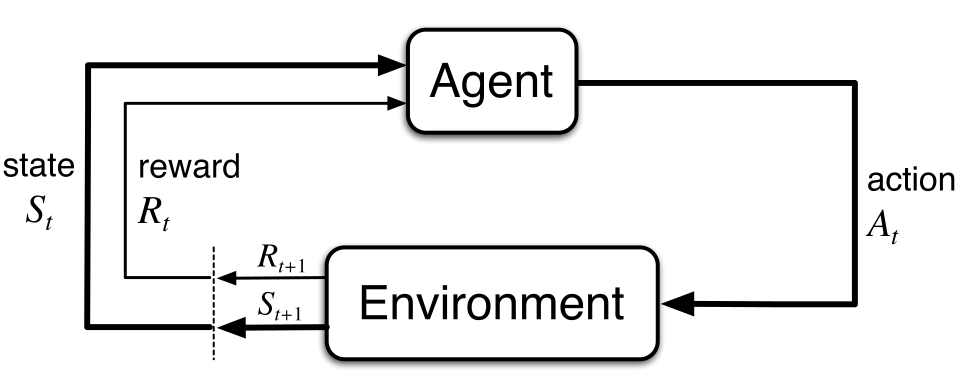
\includegraphics[scale=0.3]{./images/mdp.png}
	\caption{The agent-environment interaction in a Markov decision process.}
	\label{fig:mdp_ill}
\end{figure}


Components of RL:
\begin{itemize}
	\item An agent
	\item A policy
	\item A reward signal: what is good in an immediate sense.
	\item A value function: what is good in the long run.
	\item A model of the environment: This allows inferences to be made about how the environment will behave.
\end{itemize}
%\begin{itemize}
%	\item Agent
%	\item Action
%	\item Environment
%	\item State
%	\item The knowledge of the state is fully observable or partially observable.
%	\item Reward
%	\item Policy
%	\item Episodic task: from an initial state to a terminal state.
%	\item Continuing task: infinite horizon
%\end{itemize}


\begin{definition}[Markov Property]
	A state $S_t$ is \textbf{Markov} if and only if 
	$$P[S_{t+1}|S_t, A_t] = P[S_{t+1}|S_t, A_t, S_{t-1},A_{t-1},...]$$
\end{definition}
\begin{itemize}
	\item Actions: a mechanism to influence the environment
	\item State: specific configurations of the environment
\end{itemize}

\begin{definition}[Transition Function]
	$$p(s',r|s,a) = P(S_t=s',R_t=r|S_{t-1}=s,A_{t-1}=a)$$
\end{definition}
\begin{itemize}
	\item The way the environment changes as a response to actions is referred to as the state-transition probabilities, or more simply, the transition function, and is denoted by $T(s,a,s')$.
	\item $\sum_{r\in \mathcal{R}}\sum_{s'\in \mathcal{S}}p(s',r|s,a) = 1, \forall s \in \mathcal{S}, \forall a\in \mathcal{A}(s)$
	\item $p(s'|s,a)=P(S_t=s',R_t=r|S_{t-1}=s,A_{t-1}=a)=\sum_{r\in \mathcal{R}}p(s',r|s,a)$
\end{itemize}

\begin{definition}[Reward Hypothesis]
	All goals can be described by the maximization of expected cumulative reward.
\end{definition}
\begin{itemize}
	\item That all of what we mean by goals and purposes can be well thought of as athe maximization of the expected value of the cumulative sum of a received scalar signal (called reward).
\end{itemize}

\begin{definition}[Reward Function]
	\begin{align*}
		r(s,a)&= \mathbb{E}[R_t|S_{t-1}=s,A_{t-1}=a]\\
		&= \sum_{r\in \mathcal{R}}r\sum_{s'\in \mathcal{S}}p(s',r|s,a)
	\end{align*}
\end{definition}
\begin{itemize}
	\item $R_t\in \mathcal{R} \subset \mathbb{R}.$ Note that negative reward is still reward.
	\item The expected reward function is defined as a function that takes in a state-action pair.
	\item It is the expectation of reward at time step $t$, given the state-action pair in the previous time step.
	\item It can also be defined as a function that takes a full transition tuple $s,a,s'$.
		\begin{align*}
			r(s,a,s')&= \mathbb{E}[R_t|S_{t-1}=s,A_{t-1}=a,S_{t}=s]\\
			&= \sum_{r\in \mathcal{R}}\frac{p(s',r|s,a)}{p(s'|s,a)}
		\end{align*}
\end{itemize}




\begin{definition}[Discount Factor, $\gamma$]
	$$G_t = R_{t+1}+\gamma R_{t+2}+\gamma^2 R_{t+3}+\cdots+\gamma^{T-1} R_{t} $$
\end{definition}

\begin{itemize}
	\item The sum of all rewards obtained during the course of an episode is referred to as the return, $G_t$.
	\item Episodic tasks: $G_t = R_{t+1} + R_{t+2} + \cdots + R_{T}.$
		\begin{itemize}
			\item $G_t = R_{t+1}+\gamma G_{t+1}$
		\end{itemize}
	\item Continuing tasks: $G_t = R_{t+1} + \gamma R_{t+2} +  \gamma^2 R_{t+3} \cdots =\sum_{k=0}^{\infty} \gamma^{k} R_{t+k+1}.$
		\begin{itemize}
			\item $\gamma=0$: myopic evaluation
			\item $\gamma=1$: far-sighted evaluation
			\item Uncertainty about the future that may not be fully observed
			\item Mathematically convenient to discount rewards. 
			\item Avoid infinite returns in cyclic Markov processes.
		\end{itemize}
\end{itemize}


\section{Policies and Value Functions}
\begin{itemize}
	\item Policies are universal plans, which provides all possible plans for all states. 
		\begin{itemize}
			\item Plans are not enough to fully describe an environment in stochastic environments.
				\begin{itemize}
					\item What if an agent intends to move right, but ends up going left. Which action does the agent take?
				\end{itemize}
			\item Policies are the per-state action prescribtions.
			\item Policy can be stochastic or deterministic.
			\item A policy is a function that prescribes actions to take for a given non-terminal state.
		\end{itemize}
\end{itemize}

\subsection{The State-Value Functions}

Almost all reinforcement learning algorithms involve estimating \textit{value functions}-functions of states (or of state-action pairs) that estimate how good it is for the agent to be in a given state (or how good it is to perform a given action in a given state). The notion of ``how good'' here is defined in terms of future rewards that can be expected, or, to be precise, in terms of \textbf{expected return}. Of course, the rewards the agent can expect to receive in the futhre depend on what actions it will take. Accordingly, value functions are defined with respect to particular ways of action, called policies. 

Formally, a policy is a mapping from states to probablities of selecting each possible action. It can be defined 
$$\pi(a|s)$$


\begin{definition}[The State-Value Function, $V$]
	The state value function $v(s)$ for policy $\pi$ of an Markov Reward Process is the expected return starting from state $s$
	$$v_{\pi}(s) = \mathbb{E}_\pi[G_t|S_t=s]=\mathbb{E}_\pi \Bigg[\sum_{k=0}^\infty r^kR_{t+1+k}\Big|S_t=s\Bigg], \quad \forall s\in \mathcal{S}$$
\end{definition}

\begin{itemize}
	\item The value of a state $s$ is the expection over policy $\pi$.
	\item Reward: one-step signal that an agent gets/ Return: total discounted rewards/ Value function: expected return. 
	\item If we are given a policy and the MDP, we should be able to calculate the expected return starting from every single state. 
\end{itemize}

\begin{itemize}
	\item \textit{Bellman equation}
\begin{align*}
	v_\pi(s) &= \mathbb{E}_\pi[G_t|S_t=s]\\
	& = \mathbb{E}_\pi[R_{t+1} + \gamma G_{t+1}|S_t=s]\\
	& = \mathbb{E}_\pi[R_{t+1} + \gamma v(s_{t+1})|S_t=s]\\
	& = \sum_{a}\pi(a|s)\sum_{s',r}p(s',r|s,a)[r + \gamma v_\pi(s')]
\end{align*}
\item Starting from state $s$, the root node at the top, the agent could take any of some set of actions -- three are shown in the diagram -- based on its policy $\pi$. From each of these, the environment could respond with one of several next states, $s'$ (two are shown in the figure), along with a reward, $r$, depending on its dynamics given by the function $p$. The Bellman equation averages over all the possibilities, weighting each by its probability of occuring. \textbf{It states that the value of the start state must equal (discounted) the value of the expected next state, plus the reward expected along the way}. 
	\begin{figure}[h]
		\centering
		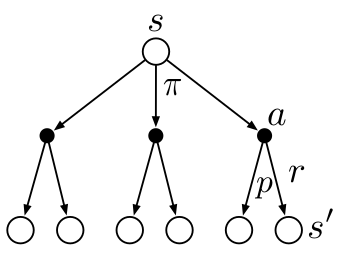
\includegraphics[scale=0.3]{./images/backup_vpi.png}
	\end{figure}
\item The derivation details are given in \Cref{appendix:bellman_equation}
\end{itemize}

\subsection{The Action-Value Function}
\begin{itemize}
	\item Another critical question that we often need to ask is not merely about the value of a state but the value of taking action $a$ at a state $s$.
	\item Which action is better under each policy?
	\item The action-value function, also known as $Q$-function or $Q^\pi(s,a)$, captures precisely this.
		\begin{itemize}
			\item The expected return if the agent follows policy $\pi$ after taking action $a$ in state $s$.
		\end{itemize}
\end{itemize}

\begin{definition}[The Action-Value Function, $Q$]
	The action-value function $q_{\pi}(s,a)$ for policy $\pi$ is the expected return starting from state $s$, tacking action $a$ under policy $\pi$
	$$q_{\pi}(s,a) = \mathbb{E}_\pi[G_t|S_t=s, A_t=a]=\mathbb{E}_\pi\Bigg[\sum_{k=0}^{\infty}\gamma^k R_{t+k+1}\Bigg| S_t=s, A_t=a\Bigg]$$
\end{definition}

\begin{itemize}
	\item The Bellman equation for action values is given by
	\begin{align*}
		q_{\pi}(s,a) &= \mathbb{E}_\pi[G_t|S_t=s, A_t=a]\\
		& = \mathbb{E}_\pi[R_{t+1} + \gamma G_{t+1}|S_t=s, A_t=a]\\
		& = \sum_{s',r}p(s',r|s,a)[r + \gamma v_\pi(s')]
	\end{align*}
	\item Notice that we do not weight over actions because we are interested only in a specific action.
	\item The state-value function can be expressed by using the action-value function as follows:
	\item The derivation is given in \Cref{appendix:bellman_equation}

The state-value function can be decomposed as follows:
\begin{align*}
	v_\pi(s) &= \mathbb{E}_{\pi}[G_t|S_t = s]\\ 
	&= \sum_{g_t} g_t\cdot P[G_t|S_t=s]\\
	&= \sum_{g_t} g_t\cdot P[G_t,S_t=s]/P[S_t=s]\\
	&= \sum_{g_t} g_t\cdot \sum_a P[G_t,S_t=s, A_t=a]/P[S_t=s]\\
	&= \sum_{g_t} g_t\cdot \sum_a \Big[P[G_t|S_t=s, A_t=a]P[S_t=s, A_t=a]\Big]/P[S_t=s]\\
	%&= \sum_{g_t} g_t \sum_a P(G_t|S_t=s, A_t=a) P(A_t=a|S_t=s)\\
	&= \sum_{g_t} g_t \sum_a P[G_t, A_t=a|S_t=s] P[A_t=a|S_t=s]\\
	&= \sum_{a} \sum_{g_t} g_t P[G_t|S_t=s, A_t=a] P[A_t=a|S_t=s]\\
	&= \sum_{a} q_\pi(s,a) \pi(a|s)
\end{align*}
Note that the expectation is parameerized $\pi$ as written in $\mathbb{E}_{\pi}$. We can also prove it by the \textit{Law of Total Expectation} \footnote{
$\mathbbm{E}[\mathbbm{E}[X|Y]] = \sum_{y}\Big[\sum_{x}x\cdot\ p(X=x|Y)\Big] p(Y=y) = \mathbbm{E}[X]$},
\begin{align*}
	v_\pi(s) &= \mathbb{E}_{\pi}[G_t|S_t = s]\\ 
	&= \mathbb{E}[\mathbb{E}_{\pi}[G_t|S_t=s, A_t=a]]\\
	&= \sum_{a} \mathbb{E}_{\pi}[G_t|S_t=s, A_t=a] P(A_t = a|S_t = s)\\
	&= \sum_{a} q_\pi(s,a) \pi(a|s)
\end{align*}
An intuitive explantation of this derivation is that the expectation depends on an action $a\sim \pi(a|s)$. We want to estimate the expected total return by the sampled action (this is because the total return is the function of $a$, implicitly). Then we need to introduce an action variable $a$ and its probability in the expression as the second line of the equation. 
\end{itemize}

\subsection{The Action-Advantage Function}

\begin{definition}[The Action-Advantage Function, $A$]
	$$a_{\pi}(s,a) = q_\pi(s,a)-v_\pi(s)$$
\end{definition}

\begin{itemize}
	\item The advantage function describes how much better it is to take action $a$ instead of following policy $\pi$. In other words, the advantage of choosing action $a$ over the default action.
\end{itemize}

\section{Optimality}

Solving a reinforcement learning task means, roughly, finding a policy that achieves a lot of reward over the long run. For finite MDPs, we can precisely define an optimal policy in the following way. Value functions define a partial ordering over policies. A policy $\pi$ is defined to be better than or equal to a policy $\pi'$ if its expected return is greater than or equal to that of $\pi'$ for all states. In other words, $\pi\geq \pi'$ if and only if $v_\pi(s)\geq v_{\pi'}(s)$ for all $s\in \mathcal{S}$. There is always at least one policy that is better than or equal to all other policies. This is an \textit{optimal policy}. The optimal state-value function, denoted $v_*$ can be defined as 


\begin{definition}[Optimal State-Value Function]
	The optimal state-value function $v_{*}(s)$ is the maximum value over all policies
	$$v_{*}(s) = \max_{\pi} v_{\pi}(s),\quad \forall s\in \mathcal{S}.$$
\end{definition}

\begin{itemize}
	\item The optimal state-value function can be obtained as follows:
%		\begin{align*}
%			v_{*}(s)&= \max_{a\in\mathcal{A}(s)} q_*(s,a)\\
%			&= \max_a \sum_{s',r}p(s',r|s,a)[r + \gamma v_*(s')]
%		\end{align*}

		\begin{align*}
			v_*(s) &= \max_{a\in \mathcal{A}(s)}q_{\pi_*}(s,a)\\
			&= \max_a \mathbb{E}_{\pi_*}[G_t| S_t=s, A_t=a]\\
			&= \max_a \mathbb{E}_{\pi_*}[R_{t+1}+\gamma G_{t+1}| S_t=s, A_t=a]\\
			&= \max_a \mathbb{E}_{\pi_*}[R_{t+1}+\gamma v_*(S_{t+1})| S_t=s, A_t=a]\\
			&= \max_a \sum_{r,s'}p(s',r|s,a)\Big[r + \gamma  v_*(s')\Big] 
	\end{align*}

\end{itemize}

\begin{definition}[Optimal Action-Value Function]
	The optimal action-value function $q_{*}(s, a)$ is the maximum value over all policies
	$$q_{*}(s,a) = \max_{\pi} q_{\pi}(s,a), \quad \forall s\in \mathcal{S} \textrm{ and } a\in \mathcal{A}.$$
\end{definition}
\begin{itemize}
	\item The optimal action-value function can be obtained as follows:
		\begin{align*}
		q_{*}(s,a) &= \mathbb{E}[R_{t+1}+\gamma v_*(S_{t+1})|S+t=s, A_t=a]\\
		&= \sum_{s',r}p(s',r|s,a)[r + \gamma \max_a q_*(s',a')]
		\end{align*}
		\begin{figure}[h]
			\centering
			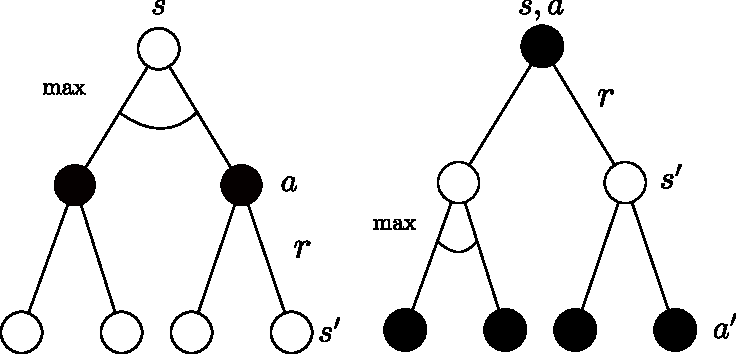
\includegraphics[scale=0.5]{./images/optimal_action.pdf}
		\end{figure}
	\item The optimal value function specifies the best possible performance in the MDP.
	\item The MDP is solved when we know the optimal value function
\end{itemize}

\begin{theorem}[Optimal Policy Theorem]
	$$\pi\geq \pi' \quad\textrm{if}\quad v_\pi(s) \geq v_{\pi'}(s), \forall s$$
	For any Markov Decision Process:
	\begin{itemize}
		\item There exists an optimal policy $\pi_*$ that is better than or equal to all other policies, $\pi_*\geq \pi, \forall \pi$
		\item All optimal policies achieve the optimal value function, $v_{\pi_*}(s) = v_*(s)$
		\item All optimal policies achieve the optimal action-value function, $q_{\pi_*}(s,a) = q_{*}(s,a)$
	\end{itemize}
\end{theorem}

An optimal policy can be found by maximizing over $q_*(s,a)$, 
\begin{align*}
	\pi_*(a|s) = 
	\begin{cases} 
		&1 \quad \textrm{if } a = \argmax_{a\in \mathcal{A}}q_*(s,a)\\
		&0 \quad \textrm{otherwise}
	\end{cases}
\end{align*}
\begin{itemize}
	\item There is always a deterministic optimal policy for any MDP
	\item If we know $q_*(s,a)$, we immediately have the optimal policy 
		\begin{itemize}
			\item Q-learning: learns Q values first
			\item Policy gradient: learns optimal policy without learning Q values
		\end{itemize}
\end{itemize}

